\chapter{Object Domain Model Translation Problem}
\label{ch:odm-transl}

The ODMTP \textit{(Object Domain Model Translation Problem)}, when talking about
Shape Expressions, is the aim to transform existing schemas, that already represent
domain models, in to object domain models. Or what it is the same, translate the ShEx
schemas to objects coded in some Object Oriented Language. \cref{fig:shex-translate-small}
represents this aim. The problem is to convert the \textit{Source} in to the \textit{Target}.

\begin{center}
	\noindent\begin{minipage}[t]{.4\textwidth}
        \begin{lstlisting}[frame=topline,numbers=left,title=\scriptsize{Person Schema (Source)},
            basicstyle=\ttfamily\scriptsize]{a}
# Prefixes...
:Person {
	:name xsd:string ;
	:knows @:Person *
}
		\end{lstlisting}
	\end{minipage}\hfill
	\begin{minipage}[t]{.5\textwidth}
        \begin{lstlisting}[language=Java, frame=t,numbers=left,title=\scriptsize{Person Java Object (Target)},
            basicstyle=\ttfamily\scriptsize]{b}
// Imports...
public class Person {
	private String name;
	private List<Person> knows;
	// Constructor...
	// Getters and Setters...
}
		\end{lstlisting}
	\end{minipage}
    \captionof{figure}{Schema modeling a \texttt{Person} in \texttt{ShExC} syntax to the left.
    And the expected translated code in \texttt{Java} to the right.}
	\label{fig:shex-translate-small}
\end{center}

This problem, with the example from \cref{fig:shex-translate-small} might seem simple to solve,
but before proposing a solution we will need to explore if the all that ShEx can express can be
translated to every object oriented programming language. For that propose we will generalize
the generated domain models to what it is known as PO \textit{(Plain Objects)} \cite{fowler1997analysis}, that is,
simple objects that do not rely on any framework. And then the main question to this problem changes to
if we can translate any Shape Expression to a Plain Object.

In order to solve that question we will need to explore and compare the expressivity of both concetps. 

% S E C T I O N   S H A P E   E X P R E S S I O N S   E X P R E S I V I T Y

\section{Shape Expressions Expressivity}
Best way to study Shape Expressions expressivity is by exploring its data model and everything that can be represented
by them, \cref{fig:shex-data-model} displays the ShEx recursive data model.

\begin{figure}
    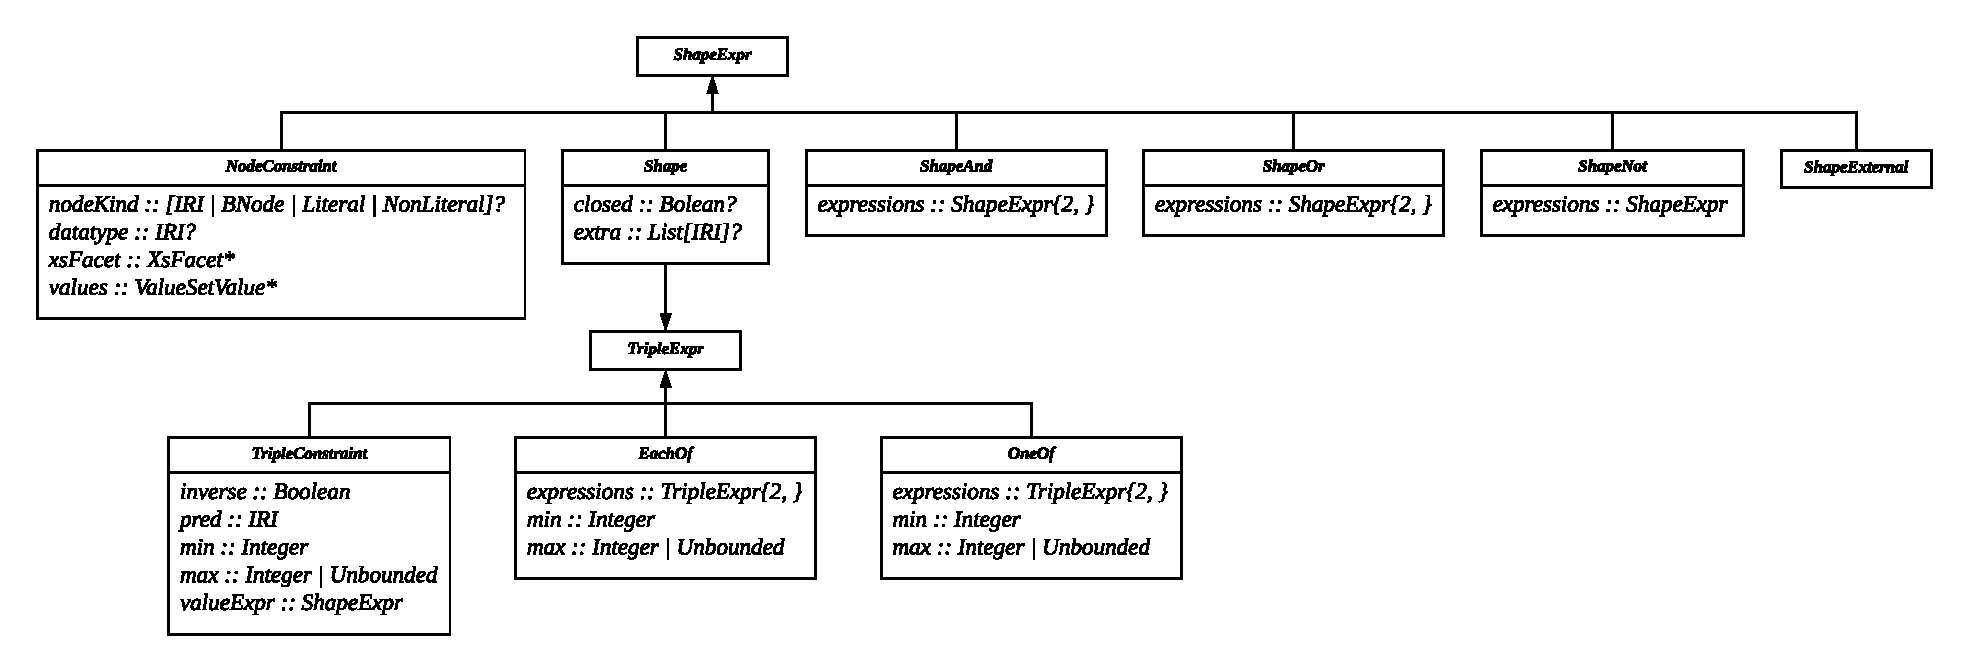
\includegraphics[width=\textwidth]{images/shape-expr-data-model.pdf}
    \centering
    \caption[ShEx data model.]{ShEx data model.}
    \label{fig:shex-data-model}
\end{figure}

As we can see from \cref{fig:shex-data-model} the data model of ShEx is hardly complicated, it contains,
conditional constraints, root node constraints, nested constraints and even logical constraints,
\cref{fig:shex-example-schemas} shows some examples of this.

When we talk about translating schemas into object domain models we are only interested in the subset of
shape expressions that are formed by a set of properties, that means the shape expressions that define constraints
for root nodes, like \cref{fig:shex-example-schemas} \textit{(a)}, won't be of our interest.

\begin{figure}
    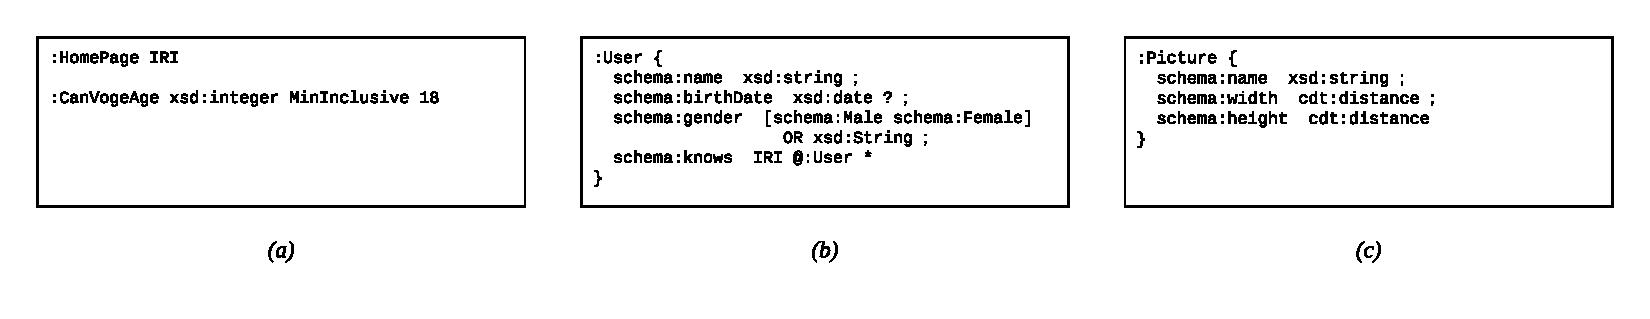
\includegraphics[width=\textwidth]{images/shex-different-expressions.pdf}
    \centering
    \caption[ShEx example schemas.]{ShEx example schemas. \textit{(a)} applies a node constraint to a root node.
    \textit{(b)} Shows how an conditional constaint can be applied to a property node. And \textit{(c)} shows how
    custom data types \texttt{ctd} can be applied to a property node.}
    \label{fig:shex-example-schemas}
\end{figure}

\subsection{Properties Set Defined Shapes}
A property set defined shape is a shape expression that it is defined as a set of properties, for example \cref{fig:shex-example-schemas}
\textit{(b)} and \textit{(c)}. This kind of shape expressions express that a node must contain the indicated properties, each one with its type.

Then, we can generalize that a shape expression is formed by the schema name and the list of constraint-annotated properties,
\cref{fig:prop-def-shape-diagram} shows the different parts that compose a property set defined shape.

\begin{figure}
    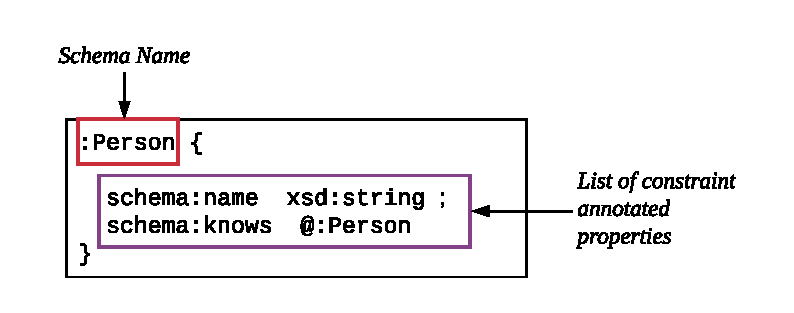
\includegraphics[scale=0.7]{images/diagram-of-shape.pdf}
    \centering
    \caption[Property set defined shape model.]{Property set defined shape model.}
    \label{fig:prop-def-shape-diagram}
\end{figure}

Furthermore, we can conclude:

\begin{partconclusion}
    The expressivity of a property set defined shape depends on the node constraints of its properties.
\end{partconclusion}

\subsection{Property Node Constraints}
The different constraints that a node might have in Shape Expressions are shown in \todo{Insertar table de
node constraints del libro de labra}.


% S E C T I O N   P L A I N   O B J E C T S   E X P R E S I V I T Y

\section{Plain Objects Expressivity}
Plain objects can be coded in any object oriented programming language, or at least in
any language that supports this paradigm. First we will explore how plain objects are 
generally coded, then how the language increases or decreases the expressivity and
finally we will generalize the core concepts that can be expressed by any plain object
codification.

\begin{figure}
    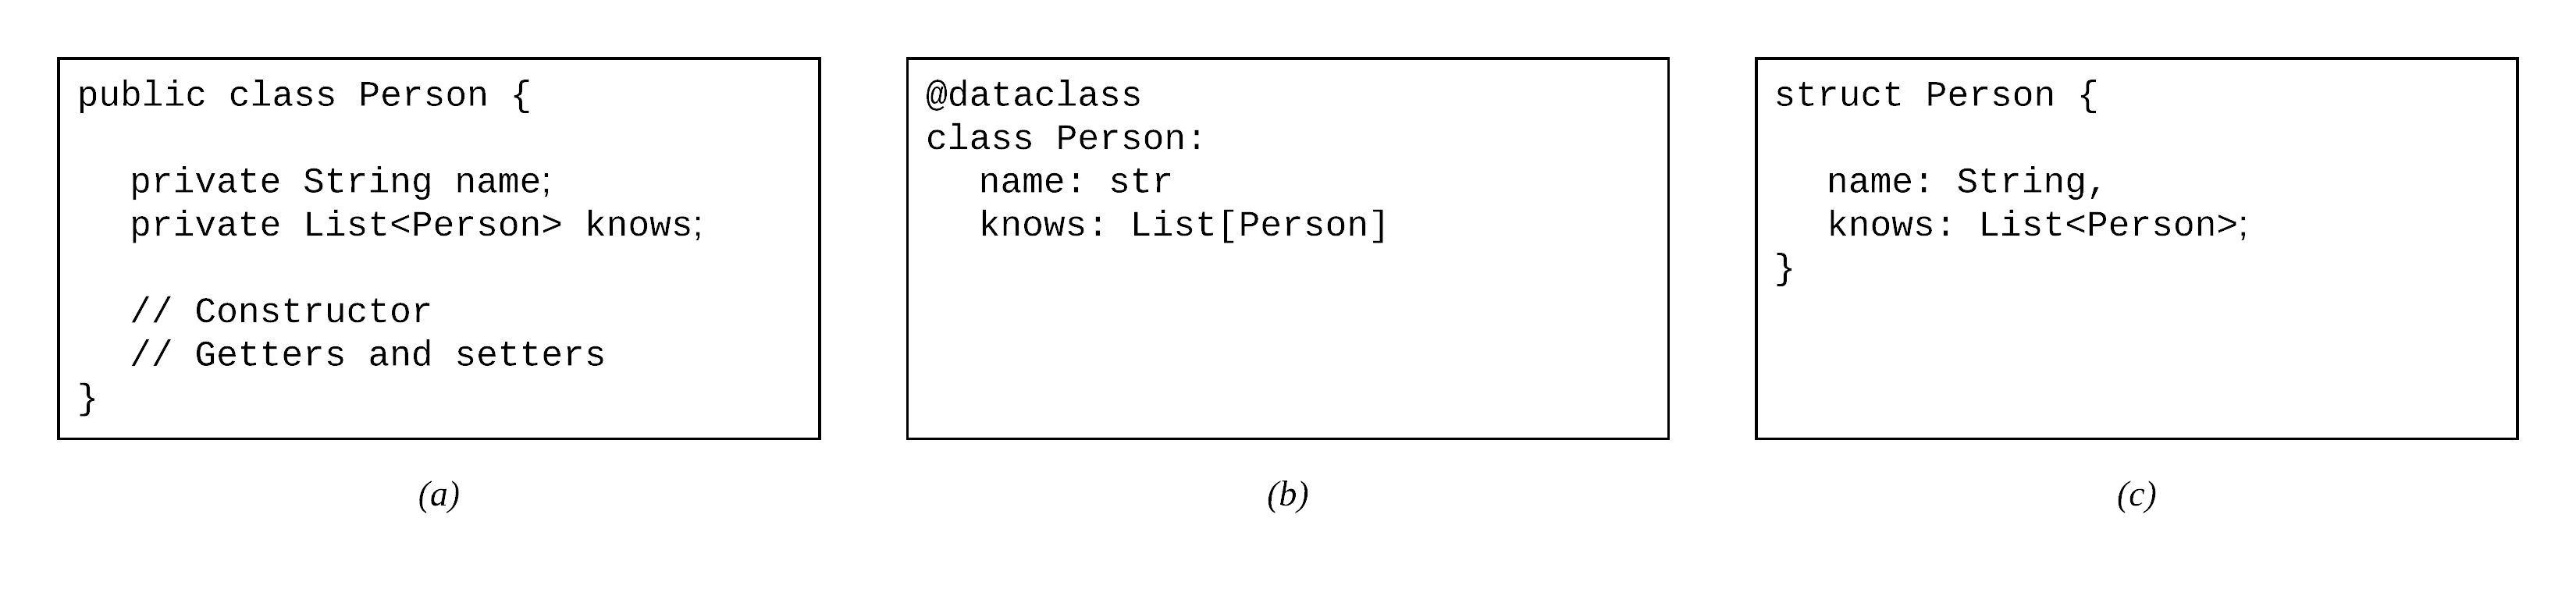
\includegraphics[width=\textwidth]{images/codings-exmaple.png}
    \centering
    \caption[Java, Python and Rust codings of Person object.]{Java, Python and Rust codings of Person object. 
    \textit{a} corresponds to Java, \textit{b} corresponds to Python and \textit{c} corresponds to Rust.}
    \label{fig:person-codings}
\end{figure}


\subsection{Plain Objects Structure}
From the existing programming languages we can infeer the general structure of plain objects. For this porpuse
we take the PYPL Index \textit{(PopularitY of Programming Language)} \footnote{\url{http://pypl.github.io/PYPL.html}}
from June 2020 and take the 2 most used programming languages that support the object oriented paradigm,
those would be Java and Python. And then, just to enlarge the scope we will take Rust because it is a new programming
language that includes lots of features.

\cref{fig:person-codings} shows three models that correspond to the codification of the Person schema from
\cref{fig:shex-translate-small}. For example if we analyze the Java fragment, that seems to be the most complex
one out of the three fragments we can see in \cref{fig:java-analysis} that it is composed by the \textit{Schema Name},
the \textit{List of Type Annotated Properties} and some \textit{Language Specific Code}. This corelates to the other
two programming languages as they also contain this three elements. Therefore after this brief analysis we can conclude:

\begin{partconclusion}
    Any Plain Object, coded in a programming language that supports the object oriented paradigm, will be composed of
    those three elements: \textbf{Schema Name}, \textbf{Type Annotated Properties} and \textbf{Language Specific Code}.
\end{partconclusion}

\begin{figure}
    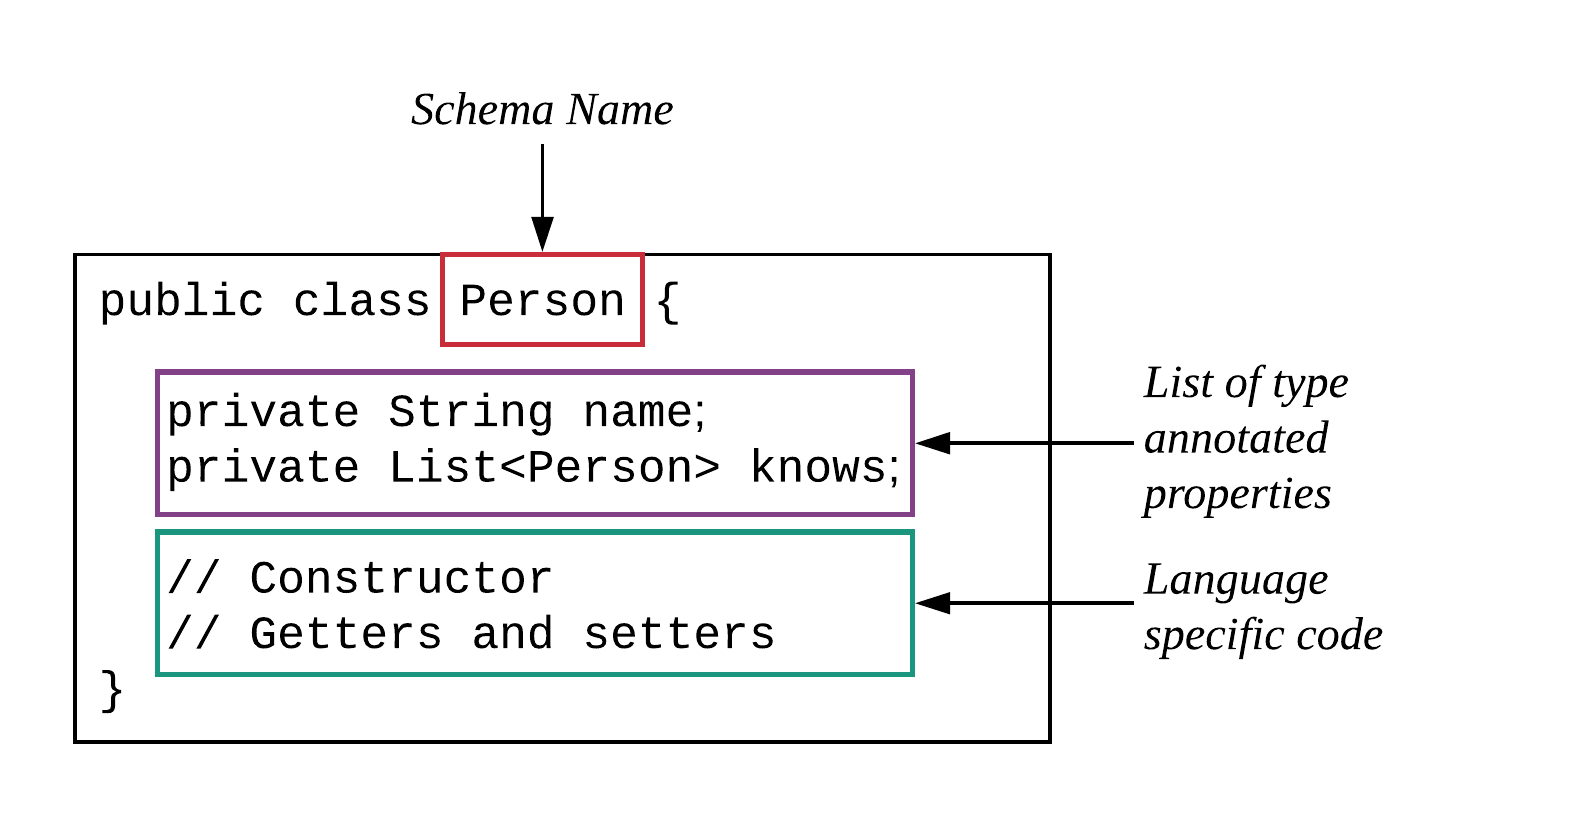
\includegraphics[scale=0.2]{images/java-analysis.png}
    \centering
    \caption[Java plain object decomposition.]{Java plain object decomposition.}
    \label{fig:java-analysis}
\end{figure}

\subsection{Plain Objects Language Expressivity Dependance}
In \cref{fig:person-codings} we can see that all of three languages use similar types to represent the Person model. But with
just one example we cannot generalize that the language does not affect the expressivity of the plain objects. In order to
test that condition and prove that the language affects or doesn't affect the expressivity of plain objects we will need first
to find two \textit{type-independent languages}.

\begin{definition}[Type-independent languages]
    Two languages $L_1$ and $L_2$ are type-independent if and only if one of the languages contains a type that cannot be
    represented by means of a linear combination of any other type of the other language.
\end{definition}

For example, lets take Java \textit{$L_1$} and Rust \textit{$L_1$}, examples \textit{(a)} and \textit{(c)} from \cref{fig:person-codings}.
Rust contains the type $Either<A,B>$, this type allows the type $A$ or $B$ and when accessed is not an $Either$ is either $A$ or $B$. In
Java there is no $Either$ type, and someone can say that we could achive a similar type by using inheritance and classes composition. But
at the end when accessed the type would be the type of the upper class. \textbf{Therefore Java and Rust are type-independent languages}.

Now in order to see if the expressivity depends on the types of a language let's assing values to Java and Rust by using the same
$Either<A,B>$ type. As can be see in \cref{fig:java-rust-comparison} Java does not allow to express the same as Rust is expressing
in this example. And therefore we can conclude that:

\begin{partconclusion}
    The expresivity of plain object is stronggly related to the build-in types that the programming language in which they are coded
    provides.
\end{partconclusion}

\begin{center}
	\noindent\begin{minipage}[t]{.4\textwidth}
        \begin{lstlisting}[language=Java,frame=topline,numbers=left,title=\scriptsize{Person Rust Struct},
            basicstyle=\ttfamily\scriptsize]{a}
stuct Person {
    name: String,
    knows: List<Person>,
    owningPet: Either<Dog,Cat>,
}
		\end{lstlisting}
	\end{minipage}\hfill
	\begin{minipage}[t]{.5\textwidth}
        \begin{lstlisting}[language=Java, frame=t,numbers=left,title=\scriptsize{Person Java Object},
            basicstyle=\ttfamily\scriptsize]{b}
// Imports...
public class Person {
    private String name;
    private List<Person> knows;
    private Pet owningPet;
    // Constructor...
    // Getters and Setters...
}
		\end{lstlisting}
	\end{minipage}
    \captionof{figure}{Rust struct modeling a \texttt{Person} to the left.
    And the most similar approximation in Java to te right. In the Java approximation the Pet class is an interface
    that it is inherited by the Cat and Dog classes, that way we allow to store in the variable \texttt{owningPet}
    values of type Cat and Dog.}
	\label{fig:java-rust-comparison}
\end{center}


\subsection{Plain Objects Expressivity Generalization}
\todo{Generalizar que un PO viene a ser una lista de propiedad valor donde lo importante son los tipos de cada lenguage,
sin embargo los tipos principales que todos los PO cumplen son los Strings, los números enteros y de coma flotante, referencias
a otros objetos y listas de los tipos anteriores.}

% S E C T I O N   C O M P A R I S O N 

\section{Shape Expressions and Plain Objects Expressivity Comparison}

Previous section cover the expressivity of Shape Expressions and Plain Objects, in this section we compare both expressivities and
expose if both expresivities are fully compatible or not.

\todo{Decir los PO presentan más restricciones que las shape expressions ya que por defecto, no permiten
tipos distintos (operaciones aritmeticológicas de tipos) y por tanto los PO permiten representar las listas de propiedades cuando
estas tienen un único tipo y su tipo es conocido (estándar).}